\documentclass{../slides}

\title{3827 OH}
\author{Eumin Hong (eh2890)}
\institute{Columbia University}
\date{February 1, 2022}

\begin{document}

\begin{frame}
    \titlepage
\end{frame}

\begin{frame}{Overview}
\begin{multicols}{2}
\tableofcontents
\end{multicols}
\end{frame}

\section{Introductions}
\subsection{About Me}
\begin{frame}{\secname: \subsecname}
    \begin{itemize}
        \item My name is Eumin Hong (UNI: eh2890)
        \item I am a junior in Columbia College studying computer science
        \item I am from New York
        \item This is my fourth time TAing for 3827 (second time with Professor Rubenstein)
        \item I took this course with Professor Kim in Fall 2020
        \begin{itemize}
            \item Took 1004, 3134, 3251 before 3827; took 3827 concurrently with 3203
        \end{itemize}
        \item Only need intro computer science course (how to code) and some high school math (mostly logic) to succeed
    \end{itemize}
\end{frame}

\subsection{About You}
\begin{frame}{\secname: \subsecname}
    \begin{itemize}
        \item Please introduce yourself and mention
        \begin{enumerate}
            \item Your name
            \item Year
            \item School
            \item Hometown
            \item Anything else that you would like to share
        \end{enumerate}
    \end{itemize}
\end{frame}

\section{Logistics}
\subsection{Course Grading}
\begin{frame}{\secname: \subsecname}
    \begin{itemize}
        \item Raw score $S$ formula:
        \begin{gather*}
            S = 0.1H + \max{\left(0.3M + 0.6F, 0.45M + 0.45F\right)} 
        \end{gather*}
        where $H$ is homework, $M$ is midterm, and $F$ is final
    \end{itemize}
\end{frame}

\subsection{Homework}
\begin{frame}{\secname: \subsecname}
    \begin{itemize}
        \item Homework will be submitted via Gradescope (entry code: 6P28R7)
        \item Scored out of $3$
        \item Relatively loose rubric -- check solutions or ask in OH for more detailed explanations
        \item Extensions are handled by me (not Professor Rubenstein)
        \begin{itemize}
            \item On the TA side, there is a spreadsheet with the latest possible submission date -- I cannot give out extensions past this date unless there is an emergency (in which case 
            \item Please contact me in advance about extensions -- psychologically, I prefer that you ask for an extension and not use it rather than have you ask me for an extension on the original due date
            \item I will grant extensions (that come in advance) in general, possible reasons include a lot of work/stress, interviews, upcoming tests/exams/essays, etc.
        \end{itemize}
    \end{itemize}
\end{frame}

\subsection{P-credit}
\begin{frame}{\secname: \subsecname}
    \begin{itemize}
        \item P-credit is a way to boost your grade, scored out of $3$
        \item Homeworks and exams count for less -- see \lstinline{3827_Lecture_00.pdf} for figures
        \item Obtain maximum P-credit by attending OH, participating, etc.
    \end{itemize}
\end{frame}

\section{OH Logistics}
\subsection{Structure}
\begin{frame}{\secname: \subsecname}
    \begin{itemize}
        \item Attendance will be taken via Zoom (either chat or participant history)
        \item After covering announcements (upcoming homeworks, exams, etc.) and notable concepts, it is whatever you would like to do
        \begin{itemize}
            \item May have additional problems to highlight edge cases/tricks, or can end early
        \end{itemize}
        \item Make use of this time and prepare your questions in advance -- can be about previous/current homeworks, current course content, etc.
    \end{itemize}
\end{frame}

\subsection{Switching OH Sections}
\begin{frame}{\secname: \subsecname}
    \begin{itemize}
        \item For both permanent and temporary switches
        \item For different TA section: email TA whose section you would like to switch to, and \textbf{CC me}
        \begin{itemize}
            \item If you do not email any TA and attend other OH section, P-credit cannot be guaranteed
            \item If you miss my OH for the week and want to attend other OH section, email me first (to acknowledge missing OH) and then email TA and CC me
            \begin{itemize}
                \item No P-credit deduction for first couple times since stuff comes up
            \end{itemize}
            \item Email in advance
        \end{itemize}
        \item For my other section: email me
        \begin{itemize}
            \item To switch to my other section is not too big of an issue; I will probably be using the same Zoom link and the sections are back-to-back
        \end{itemize}
    \end{itemize}
\end{frame}

\subsection{OH Mode}
\begin{frame}{\secname: \subsecname}
    \begin{itemize}
        \item Either online or in-person
        \item Will definitely have OH in-person for MIPS (topic after the midterm)
        \item Pros and cons to either mode
        \item Will probably go with online OH for majority of semester for notes, convenience, and health
        \item OH will not be recorded, but blank slides will be on GitHub before each OH (ideally) and notes from OH will be on GitHub
    \end{itemize}
\end{frame}

\subsection{Communication}
\begin{frame}{\secname: \subsecname}
    \begin{itemize}
        \item If you want to contact me directly, send an email to \href{mailto:eh2890@columbia.edu}{eh2890@columbia.edu}
        \begin{itemize}
            \item Please add \textbf{[3827-oh]} tag to email subject
        \end{itemize}
        \item Announcements will be via email
        \item Also open to a group messaging system for OH (will send announcements here as well if created)
        \begin{itemize}
            \item Options include Slack, etc.
            \item Will probably merge my OH sections
        \end{itemize}
    \end{itemize}
\end{frame}

\subsection{Feedback}
\begin{frame}{\secname: \subsecname}
    \begin{itemize}
        \item This semester, I will be trying anonymous feedback
        \item Form: \url{https://forms.gle/cnUmKVNYN7WvRbHA6}
        \item You can also provide feedback via email or include your name in the form
    \end{itemize}
\end{frame}

\subsection{Resources}
\begin{frame}{\secname: \subsecname}
    \begin{itemize}
        \item OH GitHub: \url{https://github.com/eh2890/CSEE_W3827_S2022}
        \begin{itemize}
            \item Will have course lectures slides, OH slides, OH notes, etc. here
        \end{itemize}
        \item All OH Sections: \url{http://uribe.cs.columbia.edu/sched/assigned-slotorder.html}
        \item My OH Sections:
        \begin{itemize}
            \item Section \#11: Tuesday 3pm
            \item Section \#10: Tuesday 4pm
        \end{itemize}
        \item Course Google Calendar: \url{https://calendar.google.com/calendar/u/0/embed?src=16uc8kberc2b6dtltq6e49dv3k@group.calendar.google.com&ctz=America/New_York}
        \begin{itemize}
            \item Additional OH will be posted here and also announced
        \end{itemize}
    \end{itemize}
\end{frame}

\section{Notable Concepts}
\subsection{Binary Syntax}
\begin{frame}{\secname: \subsecname}
    When writing in binary, syntax can help everyone trying to read it. We usually deal with binary numbers that have a number of bits divisible by 4 (e.g. 8-bit, 32-bit, 64-bit). Compare the (identical in value) two 32-bit numbers:
    \begin{center}
        \lstinline{00000000110111111111001101011101}\\
        \lstinline{0000 0000 1101 1111 1111 0011 0101 1101}
    \end{center}
    The first is hard to read. The second is easier to read. Group bits by four for readability -- it's easier to see when you've missed a bit, and it's easier for me to grade.
\end{frame}

\subsection{Binary Representation}
\begin{frame}{\secname: \subsecname}
    What is the value of the 8-bit number \lstinline{1001 0110}? Is it $150$ (unsigned)? Is it $-22$ (signed magnitude)? Is it $-105$ (1's complement)? Is it $-106$ (2's complement)? Is it \^{u} (ASCII)?\\
    Binary numbers are just an ordering of bits; their meaning comes from how they are interpreted.\\
    The LSB is bit $0$, the MSB is bit $k-1$ for a $k$-bit binary number. For review:
    \begin{itemize}
        \item Unsigned magnitude: bit $i$ is $2^i$, nothing special about MSB
        \item Signed magnitude: MSB does not have value, simply indicates the sign of the number
        \item 1's complement: MSB indicates sign -- if MSB is $1$, then flip all the bits and negate the result
        \item 2's complement: MSB indicates sign -- if MSB is $1$, then flip all the bits and add $1$
    \end{itemize}
    Note: signed magnitude and 1's complement result in two ways to represent $0$ (think $+0$ and $-0$).
\end{frame}

\subsection{2's Complement Subtraction}
\begin{frame}{\secname: \subsecname}
    Subtracting is the same as adding a negative number:
    \begin{gather*}
        X - Y = X + (-Y)
    \end{gather*}
\end{frame}

\subsection{Detecting Overflow}
\begin{frame}{\secname: \subsecname}
    \begin{itemize}
        \item Unsigned
        \begin{itemize}
            \item Addition: overflow occurs if final carry is $1$ 
            \item Subtraction: overflow in $X - Y$ occurs if $X < Y$
        \end{itemize}
        \item 2's complement
        \begin{itemize}
            \item Overflow occurs if the two final carries (most significant) do not match
        \end{itemize}
    \end{itemize}
\end{frame}

\subsection{Boolean Complement Syntax}
\begin{frame}{\secname: \subsecname}
    Consider the expressions below:
    \begin{align*}
        \overbar{XY} &= \overbar{X} + \overbar{Y}\\
        \overbar{X}\overbar{Y} &= \overbar{X + Y}
    \end{align*}
    The expressions $\overbar{XY}$ and $\overbar{X}\overbar{Y}$ are different -- the space between the complement bars is crucial.\\
\end{frame}

\subsection{XOR}
\begin{frame}{\secname: \subsecname}
    For two inputs, the XOR operator ensures that \textbf{exactly one} of the inputs is $0$ (and \textbf{exactly one} of the inputs is $1$ as well). Some definitions:
    \begin{multicols}{2}
    \begin{figure}[H]
        \centering
        \begin{table}[H]
        \begin{tabular}{|c|c|c|}
        \hline
        $X$ & $Y$ & $X\oplus Y$ \\ \hline\hline
        $0$ & $0$ & $0$ \\ \hline
        $0$ & $1$ & $1$ \\ \hline
        $1$ & $0$ & $1$ \\ \hline
        $1$ & $1$ & $0$ \\ \hline
        \end{tabular}
        \end{table}
    \end{figure}
    $$X\oplus Y = X\overbar{Y} + \overbar{X}Y$$
    \end{multicols}
    Important properties:
    \begin{itemize}
        \item Commutativity: $X\oplus Y = Y\oplus X$
        \item Associativity: $X\oplus (Y\oplus Z) = (X\oplus Y) \oplus Z$
        \item Identity: $X\oplus 0 = X$
        \item Inverse: $X\oplus X = 0$
        \item Negation: $X\oplus Y = \overbar{X} \oplus \overbar{Y} \neq \overbar{X\oplus Y} = X\overbar{\oplus}Y$
    \end{itemize}
    It follows that for $n$ inputs, $X_1\oplus \cdots \oplus X_n = 1$ for an odd number of $X_i$.
\end{frame}

\subsection{XNOR}
\begin{frame}{\secname: \subsecname}
    If 2-input XOR checks for inequality, XNOR checks for equality:
    \begin{figure}[H]
        \centering
        \begin{table}[H]
        \begin{tabular}{|c|c|c|c|}
        \hline
        $X$ & $Y$ & $X\oplus Y$ & $X\overbar{\oplus} Y$ \\ \hline\hline
        $0$ & $0$ & $0$ & $1$\\ \hline
        $0$ & $1$ & $1$ & $0$\\ \hline
        $1$ & $0$ & $1$ & $0$\\ \hline
        $1$ & $1$ & $0$ & $1$\\ \hline
        \end{tabular}
        \end{table}
    \end{figure}
    If we perform bit-wise XNOR on two $k$-bit numbers $X$ and $Y$ and then AND all the results, we can check if $X == Y$:
    \begin{figure}[H]
        \centering
        \begin{tikzpicture}[circuit logic US, label distance=2mm]\centering
            \node (xmsb) at (0, 2) {$X_{k-1}$};
            \node (ymsb) at (0, 1.5) {$Y_{k-1}$};
            \node () at (0, 1) {$\vdots$};
            \node (x0) at (0, 0.25) {$X_0$};
            \node (y0) at (0, -0.25) {$Y_0$};
            \node[xnor port, draw, scale=0.89] at (2, 1.75) (xnor1){};
            \node (dots) at (2, 1) {$\vdots$};
            \node[xnor port, draw, scale=0.89] at (2, 0) (xnor0){};
            \draw (xmsb) -- (xnor1.in 1);
            \draw (ymsb) -- (xnor1.in 2);
            \draw (x0) -- (xnor0.in 1);
            \draw (y0) -- (xnor0.in 2);
            \node[and gate, draw, logic gate inputs=nnn] at (3, 0.875) (and){};
            \draw (xnor1.out) -| (2.5, 1.75) |- (and.input 1);
            \draw (2.3, 0.875) -- (and.input 2);
            \draw (xnor0.out) -| (2.5, 0) |- (and.input 3);
            \node (f) at (4, 0.875) {$F$};
            \draw (and.output) -- (f);
        \end{tikzpicture}
    \end{figure}
\end{frame}

\subsection{Drawing Circuits}
\begin{frame}{\secname: \subsecname}
    Be sure that your circuits are not ambiguous. Use dots to indicate which wires are connected, like so:\footnote{From Lecture 02, Slide 35}
    \begin{figure}[H]
        \centering
        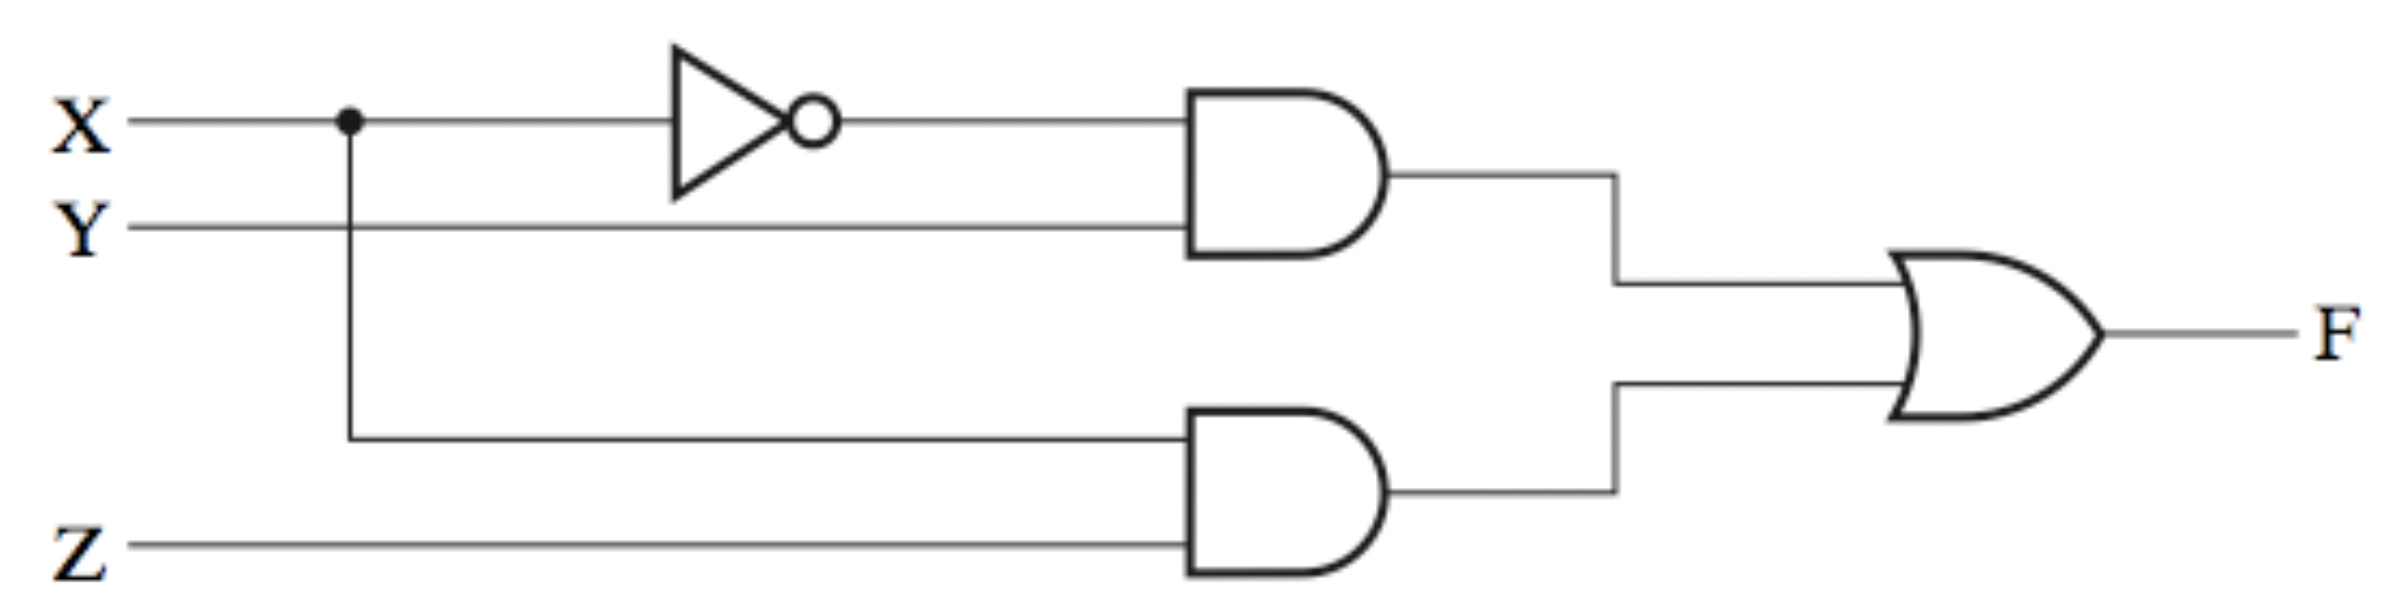
\includegraphics[width = 6cm]{img/circuit.png}
    \end{figure}
    You may consider something like:
    \begin{figure}[H]
    \centering
    \begin{tikzpicture}[circuit logic US, label distance=2mm]\centering
        \node (x) at (0, 2) {$X$};
        \node (y) at (0, 1.5) {$Y$};
        \node (z) at (0, 1) {$Z$};
        \draw (x) -- (7, 2);
        \draw (y) -- (7, 1.5);
        \draw (z) -- (7, 1);
        \node[or gate, draw, rotate = -90] at (2, 0.25) (or){};
        \node[xor gate, draw, rotate = -90] at (4, 0.25) (xor){};
        \node[and gate, draw, logic gate inputs=nnn, rotate = -90] at (6, 0.25) (and){};
        \draw (x) -| (or.input 2);
        \draw (y) -| (or.input 1);
        \draw (x) -| (xor.input 2);
        \draw (z) -| (xor.input 1);
        \draw (x) -| (and.input 3);
        \draw (y) -| (and.input 2);
        \draw (z) -| (and.input 1);
        \draw[black,fill=black] (1.9, 2) circle (0.05) node {};
        \draw[black,fill=black] (2.1, 1.5) circle (0.05) node {};
        \draw[black,fill=black] (3.9, 2) circle (0.05) node[anchor=south east] {};
        \draw[black,fill=black] (4.1, 1) circle (0.05) node[anchor=south east] {};
        \draw[black,fill=black] (5.85, 2) circle (0.05) node[anchor=south east] {};
        \draw[black,fill=black] (6, 1.5) circle (0.05) node[anchor=south east] {};
        \draw[black,fill=black] (6.15, 1) circle (0.05) node[anchor=south east] {};
        \node (a) at (2, -0.75) {$A$};
        \node (b) at (4, -0.75) {$B$};
        \node (c) at (6, -0.75) {$C$};
        \draw (or.output) -- (a);
        \draw (xor.output) -- (b);
        \draw (and.output) -- (c);
    \end{tikzpicture}
    \end{figure}
\end{frame}

\section{Homework 1}
\subsection{Problem 1}
\begin{frame}{\secname: \subsecname}
    Assume an architecture where all numbers are to be represented using 8 bits. What are the (base 10) values of the 8-bit binary numbers when interpreted using (i) unsigned, (ii) signed magnitude, (iii) 1’s complement, (iv) 2’s complement form:
    \begin{enumerate}[(a)]
        \item $00110011$
        \item $10000000$
        \item $11111111$
        \item $10011011$
        \item $10001010$
    \end{enumerate}
\end{frame}

\subsection{Problem 2}
\begin{frame}{\secname: \subsecname}
    Convert the following (base 10) numbers to their binary representation using 8-bit (i) signed magnitude, (ii) 1’s complement, (iii) 2’s complement forms:
    \begin{enumerate}[(a)]
        \item $-1$
        \item $-15$
        \item $-67$
        \item $-127$
    \end{enumerate}
\end{frame}

\subsection{Problem 3}
\begin{frame}{\secname: \subsecname}
    For each pair of $x$ and $y$ below, convert $x$ and $y$ to their 8-bit 2’s-complement forms, subtract $y$ from $x$ (so you need to negate $y$ and then add). Indicate whether an overflow occured (and show clearly how you know), and convert the solution back to base 10 (even when an overflow occured and the solution is wrong, i.e., your answer should fit in the 8-bit representation of that form.).
    \begin{enumerate}[(a)]
        \item $x = 10, y = -13$
        \item $x = 117, y = 35$
        \item $x = 117, y = -35$
        \item $x = -117, y = 35$
        \item $x = -117, y = 11$
    \end{enumerate}
\end{frame}

\subsection{Problem 4}
\begin{frame}{\secname: \subsecname}
    Given the bit pattern $1010\ 1101\ 0001\ 0000\ 0000\ 0000\ 0000\ 0010$, what does it represent, assuming that it is
    \begin{enumerate}[(a)]
        \item a two's complement integer?
        \item an unsigned integer?
        \item a single precision (32-bit) floating-point number?
    \end{enumerate}
\end{frame}

\subsection{Problem 5}
\begin{frame}{\secname: \subsecname}
    Represent the following numbers, given here in binary form, as floating point numbers using IEEE 754 floating- point standard representation:
    \begin{enumerate}[(a)]
        \item $11010.1110$
        \item $-11011.10$
        \item $0.000101$
        \item $-1.010101$
        \item $10000000010$
    \end{enumerate}
\end{frame}

\end{document}
